\documentclass{article}
\usepackage{graphicx}
\usepackage{amsmath}
\usepackage{pgfplots}
\usepackage{physics}
\usepackage{cancel}
\usepackage{bigints}
\usepackage{enumitem}
\usepackage{txfonts}
\usepackage[normalem]{ulem}

\newcommand{\g}{\text{g}}
\newcommand{\kilo}{\text{k}}
\newcommand{\m}{\text{m}}
\newcommand{\centi}{\text{c}}
\newcommand{\s}{\text{s}}
\newcommand{\N}{\text{N}}
\newcommand{\J}{\text{J}}
\newcommand{\C}{\text{C}}
\newcommand{\V}{\text{V}}
\newcommand{\A}{\text{A}}
\newcommand{\Ohm}{\text{\Omega}}

\pgfplotsset{compat=1.18}

\pgfplotsset{compat=1.18}

\usepackage[a4paper, top=1cm, bottom=2cm, left=2cm, right=2cm, includehead, includefoot]{geometry}



\begin{document}

\noindent
Physics 4B - Electromagnetism \hfill Prof. Alfred Cauthen
\noindent\rule{\textwidth}{0.4pt}

\begin{center}
    \textbf{\LARGE Homework 7} \\
    \vspace{12pt}
    \large Aaron W. Tarajos \\
    \textit{\today}
\end{center}

\noindent\rule{\textwidth}{0.4pt}

\section*{Question 2}
Figure 24-25 shows three sets of cross sections of equipotential surfaces in uniform electric fields; all three cover the same size region of space. The electric potential is indicated for each surface. (a) Rank the surfaces according to the magnitude of the electric field, greatest first. (b) In which is the electric field directed down the page?

\begin{figure}[h]
	\centering
	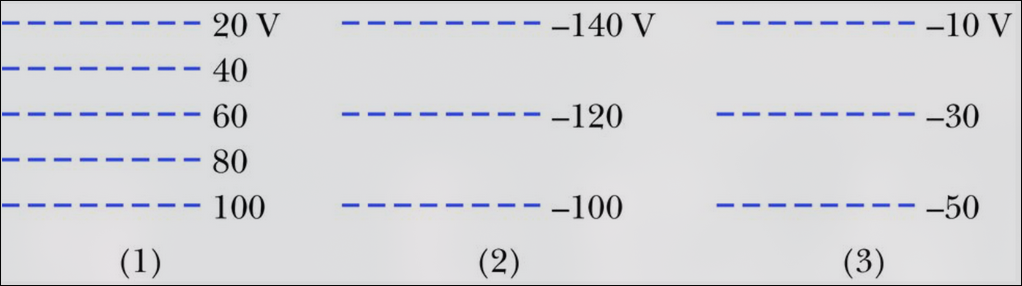
\includegraphics[width=0.5\textwidth]{image.png}
	\caption{Figure 24-25}
\end{figure}

\subsection*{Solution}
The magnitude of the field for a uniform field is given by;

\begin{equation}
	E = \frac{\Delta V}{\Delta s}
\end{equation}
but we don't really care about $\Delta s$ because we are looking at magnitude, so we have;

\begin{align*}
	\Delta V_1 &= 100 - 20 = 80 \V \\
	\Delta V_2 &= -100 - (-140) = 40 \V \\
	\Delta V_3 &= -50 - (-10) = 40 \V
\end{align*}
therefore, $1 > 2 = 3$.

\section*{Question 3}
Figure 24-26 shows four pairs of charged particles. For each pair, let
$V = 0$ at infinity and consider $V_\text{net}$ at points on the $x$ axis. For which pairs
is there a point at which $V_\text{net} = 0$ (a) between the particles and (b) to the right of the particles? (c) At such a point is $E_\text{net}$ due to the particles equal to zero? (d) For each pair, are there off-axis points (other than at infinity) where $V_\text{net} = 0$?

\begin{figure}[h]
	\centering
	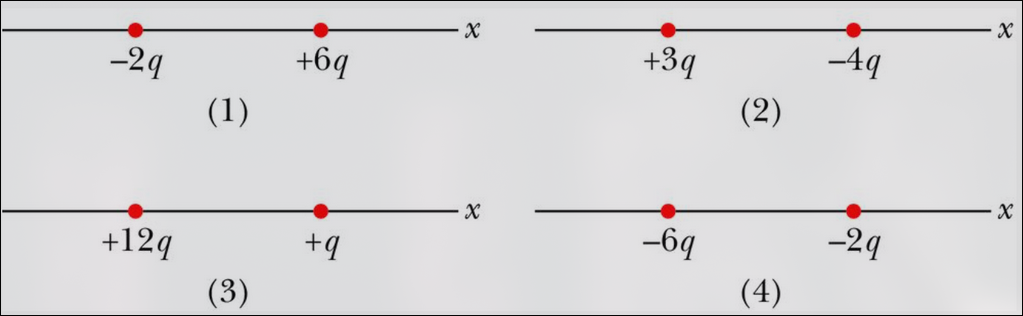
\includegraphics[width=0.5\textwidth]{image-2.png}
	\caption{Figure 24-26}
\end{figure}

\subsection*{Solution}
The electric potential from a point charge is given by;
\begin{equation}
    V = \frac{kq}{r}
\end{equation}
which we then sum across all charges to find the net electric potential.\\
\textbf{Part a:}
\begin{align*}
	V_1 &= \frac{-2qk}{r_1} + \frac{k6q}{r_2} \implies \frac{r_2}{r_1} = 3\\
	V_2 &= \frac{k3q}{r_1} + \frac{-4qk}{r_2} \implies \frac{r_2}{r_1} = \frac{4}{3}\\
	V_3 &= \frac{k12q}{r_1} + \frac{kq}{r_2} \implies \frac{r_2}{r_1} = -11\\
	V_4 &= \frac{-6qk}{r_1} + \frac{-2qk}{r_2} \implies \frac{r_2}{r_1} = -3
\end{align*}
these equations give the necessary ratios of $r_2$ to $r_1$ to achieve a net potential of 0 between the charges. Because we cannot have a negative distance, we can discard $V_3$ and $V_4$.\\[10pt]
\textbf{Part b:}
Looking at a point to the right of the particles, we can disregard $V_3$ and $V_4$ because nothing has changed, the charges are still the same sign and so the potential cannot sum to zero. For $V_1$ and $V_2$, notice that both of those values are greater than 1, which means that $r_2$ must be greater than $r_1$ which is not possible to the right of the particles. So there are no points to the right of the particles where the potential is zero.\\[10pt]
\textbf{Part c:}
No because the electric field is;
\begin{align*}
	E &= -\frac{dV}{dr} \\
	&= \frac{kq_1}{r_1^2} + \frac{kq_2}{r_2^2} \\
\end{align*}
and that will not be zero for the same ratio of $r_2$ to $r_1$ as in part a.\\[10pt]
\textbf{Part d:}
Yes, there are many off-axis points as long as the particles have opposite charges and the ratio of the distances between the points are such that it cancels any assymetry in the charge magnitudes.

\section*{Question 9}
Figure 24-26 shows four pairs of charged particles with identical separations. (a) Rank the pairs according to their electric potential energy (that is, the energy of the two-particle system), greatest(most positive) first. (b) For each pair, if the separation between the particles is increased, does the potential energy of the pair increase or decrease?

\subsection*{Solution}
\textbf{Part a:} Since the distance between the charges is fixed, only the net charge of the system matters. Which gives us the order; $3 > 1 > 2 > 4$.\\[10pt]
\textbf{Part b:} (1) Decreases, (2) Increases, (3) Decreases, (4) Increases. This is because the potential energy is given by;
\begin{equation*}
    U = \frac{kq_1q_2}{r}
\end{equation*}
so if the potential is positive it decreases and if the potential is negative it increases.

\section*{Question 11}
Figure 24-32 shows a thin, uniformly charged rod and three points at the same distance $d$ from the rod. Rank the magnitude of the electric potential the rod produces at those three points, greatest first.

\begin{figure}[h]
	\centering
	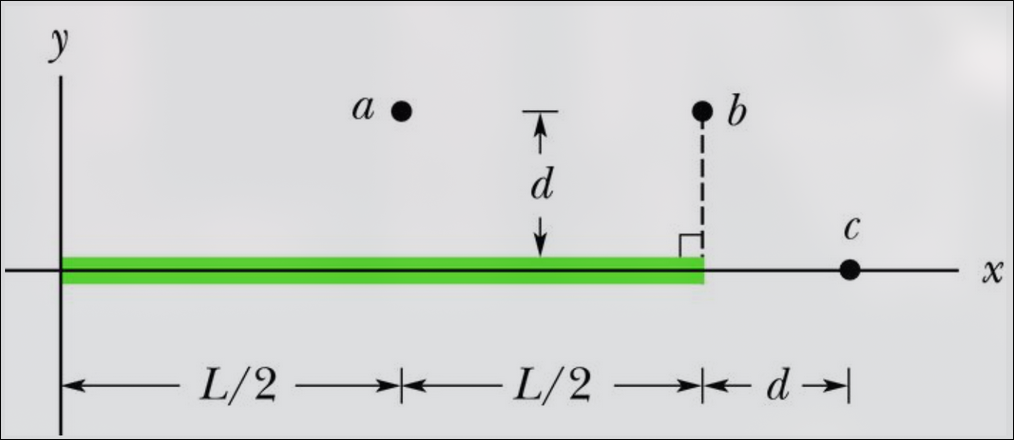
\includegraphics[width=0.5\textwidth]{image-3.png}
	\caption{Figure 24-32}
\end{figure}

\subsection*{Solution}
The ranking of the electric potential is $a > b > c$ because the electric potential is given by;
\begin{equation*}
    V = \frac{k\lambda}{r}
\end{equation*}
and because $a$ is the closes to the majority of the rod it has the highest potential, followed by $b$ and then $c$ is the farthest away from all points so it has the lowest potential.

\section*{Question 12}
In Fig. 24-33, a particle is to be released at rest at point $A$ and then is to be accelerated directly through point $B$ by an electric field. The potential difference between points $A$ and $B$ is 100 V. Which point should be at higher electric potential if the particle is (a) an electron, (b) a proton, and (c) an alpha particle (a nucleus of two protons and two neutrons)? (d) Rank the kinetic energies of the particles at point $B$, greatest first.

\begin{figure}[h]
	\centering
	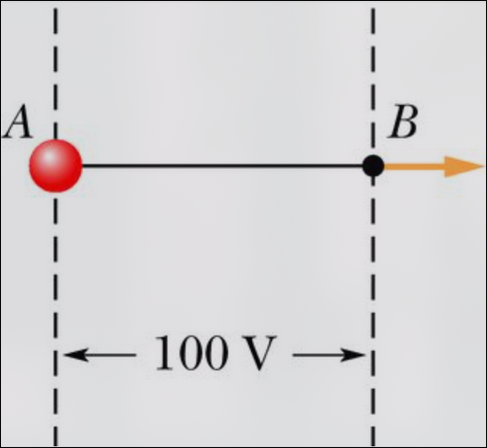
\includegraphics[width=0.5\textwidth]{image-4.png}
	\caption{Figure 24-33}
\end{figure}

\subsection*{Solution}
The electron has the highest potential at point $B$ because the it will feel force in the opposite direction of the field lines. The proton feels the highest potential at point $A$ because the force will be in the same direction as the field lines. The same goes for the alpha particle. \\[10pt]
\textbf{Part d:} The kinetic energy of a particle is given by $qV$. The proton and the electron have the same magnitude of charge just different signs, so they will have the same kinetic energy. The alpha particle has twice the charge of the proton so it will have the highest kinetic energy. $K_\alpha > K_p = K_e$.


\section*{Problem 6}
When an electron moves from $A$ to $B$ along an electric field line in Fig. 24-34, the electric field does $3.94 \times 10^{-19}$ J of work on it. What are the electric potential differences (a) $V_B - V_A$, (b) $V_C - V_A$, and (c) $V_C - V_B$?

\begin{figure}[h]
	\centering
	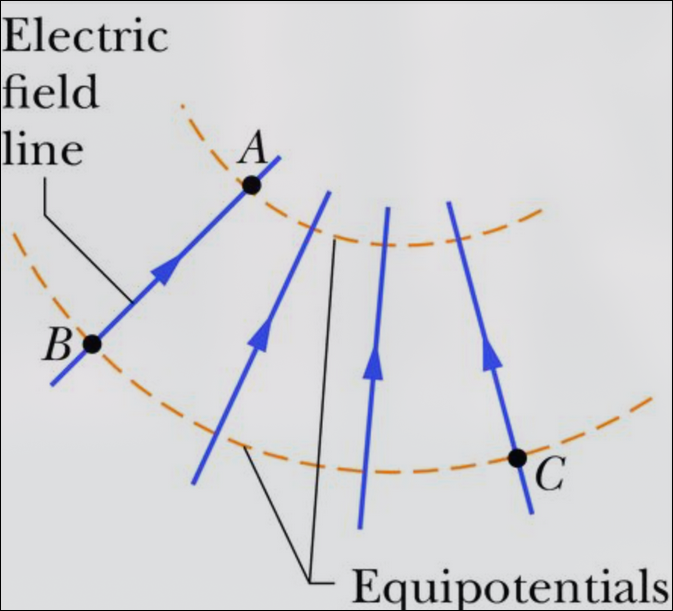
\includegraphics[width=0.5\textwidth]{image-5.png}
	\caption{Figure 24-34}
\end{figure}

\subsection*{Solution}
\textbf{Part a:}
\begin{align*}
	V_B - V_A &= \frac{W}{q} \\
	&= \frac{3.94 \times 10^{-19}}{-1.602 \times 10^{-19}} \\
	&= \boxed{-2.46 \V}
\end{align*}
\textbf{Part b:} It is the same as part a because there is no work done along the equipotential, therefore only the difference in potential from $B$ to $A$ matters. \\[10pt]
\textbf{Part c:} Again the work along an equipotential is zero so the difference in potential is zero.

\section*{Problem 8}
A graph of the $x$ component of the electric field as a function of $x$ in a region of space is shown in Fig. 24-35. The scale of the vertical axis is set by $E_x = 20.0$ N/C. The $y$ and $z$ components of the electric field are zero in this region. If the electric potential at the origin is $V_0 = 10$ V, (a) what is the electric potential at $x = 2.0$ m, (b) what is the greatest positive value of the electric potential for points on the $x$ axis for which $0 \leq x \leq 6.0$ m, and (c) for what value of $x$ is the electric potential zero?

\begin{figure}[h]
	\centering
	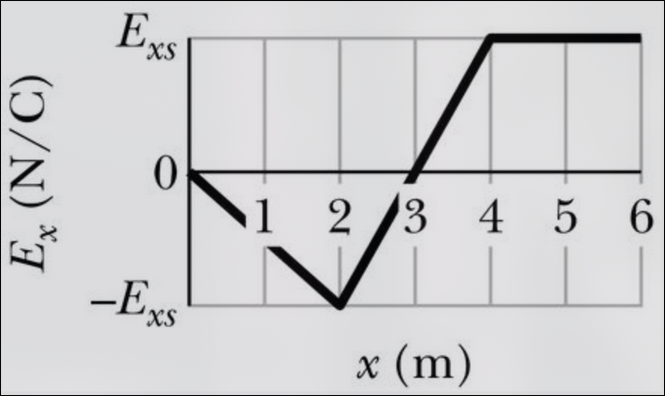
\includegraphics[width=0.5\textwidth]{image-6.png}
	\caption{Figure 24-35}
\end{figure}

\subsection*{Solution}
\textbf{Part a:}
given the initial potential, we just have to find the area under the curve(really just the area of a triangle but I like showing the general case) from $x=0$ to $x=2$.
\begin{align*}
	V_f - V_i &= \int_i^f E_x dx \\
	V_f - 10&= \int_0^2 \frac{20}{2} dx \\
	V_f - 10 &= 20 \\
	V_f &= \boxed{30 \V}
\end{align*}
\textbf{Part b:} The maximum potential occurs where the slope of the electric field is the greatest, which is at $x=3$.
\begin{align*}
	V_f - V_i &= \int_i^f E_x dx \\
	V_f - 10&= \int_0^3 \frac{20}{2} dx \\
	V_f - 10 &= 30 \\
	V_f &= \boxed{40 \V}
\end{align*}
\textbf{Part c:} The potential is zero where the area under the curve is equal to the initial potential.
\begin{align*}
	20(x-4)&=30 \\
	20x - 80 &= 30 \\
	x &= \boxed{5.5 \m}
\end{align*}

\section*{Problem 10}
Two uniformly charged, infinite, nonconducting planes are parallel to a $yz$ plane and positioned at $x = -50$ cm and $x = +50$ cm. The charge densities on the planes are $-50$ nC/m$^2$ and $+25$ nC/m$^2$, respectively. What is the magnitude of the potential difference between the origin and the point on the $x$ axis at $x = +80$ cm? (Hint: Use Gauss' law.)

\subsection*{Solution}
\begin{align*}
	\Delta V &= \int_i^f E_x \vec{ds} \\
	&= \int_0^{80} \vec{E} \cdot \vec{ds} \\
	&= \int_0^{50} \vec{E} \cdot \vec{ds} + \int_{50}^{80} \vec{E} \cdot \vec{ds} \\
	&= \vec{E}_1 - \vec{E}_2 \int_0^{50} \vec{ds} + \vec{E}_1 + \vec{E}_2 \int_{50}^{80} \vec{ds} \\
	&= \left(\vec{E}_1 - \vec{E}_2\right)50 + 30\left(\vec{E}_1 + \vec{E}_2\right) \\
	&= 80\vec{E}_1 - 20\vec{E}_2 \\
	&= 80\left(\frac{\sigma_1}{2\epsilon_0}\right) + 20\left(\frac{\sigma_2}{2\epsilon_0}\right) \\
	&= 80\left(-50 \times 10^{-9} \frac{1}{2\epsilon_0}\right) + 20\left(25 \times 10^{-9} \frac{1}{2\epsilon_0}\right) \\
	&= 0.4\left(\frac{1}{\epsilon_0}\right) \left(-50 \times 10^{-9}\right) + 0.1\left(\frac{1}{\epsilon_0}\right) \left(25 \times 10^{-9}\right) \\
	&= \boxed{1977.401\ \J/\C}
\end{align*}

\section*{Problem 16}
Figure 24-37 shows a rectangular array of charged particles a fixed in place, with distance a = 39.0 cm and the charges shown as integer multiples of $q_1 = 3.40$ pC and $q_2 = 6.00$ pC. With $V = 0$ at infinity, what is the net electric potential at the rectangle's center?

\begin{figure}[h]
	\centering
	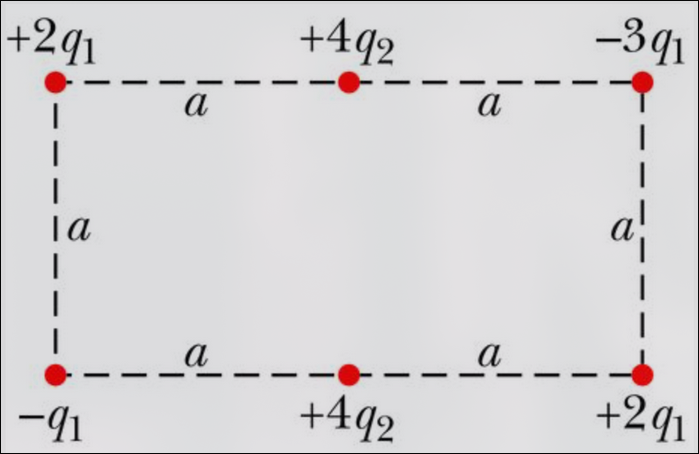
\includegraphics[width=0.5\textwidth]{image-7.png}
	\caption{Figure 24-37}
\end{figure}

\subsection*{Solution}
From the symmetry the corners all cancel out and so we just have to find the potential from the two middle charges.
\begin{align*}
	V &= \frac{4kq_2}{a/2} + \frac{4kq_2}{a/2} \\ 
	&= \frac{8kq_2}{a} + \frac{8kq_2}{a} \\
	&= \frac{16kq_2}{a} \\
	&= \frac{(16) (8.99 \times 10^9) (6 \times 10^{-12})}{0.39} \\
	&= \boxed{2.212\ \J/\C}
\end{align*}

\section*{Problem 30}
The smiling face of Fig. 24-49 consists of three items:\\
1. a thin rod of charge -3.0 $\mu$C that forms a full circle of radius 6.0 cm;\\
2. a second thin rod of charge 2.0 $\mu$C that forms a circular arc of radius 4.0 cm, subtending an angle of 90° about the center of the full circle;\\
3. an electric dipole with a dipole moment that is perpendi­cular to a radial line and has a magnitude of $1.28 \times 10^{-21}$ C · m.
What is the net electric potential at the center?

\begin{figure}[h]
	\centering
	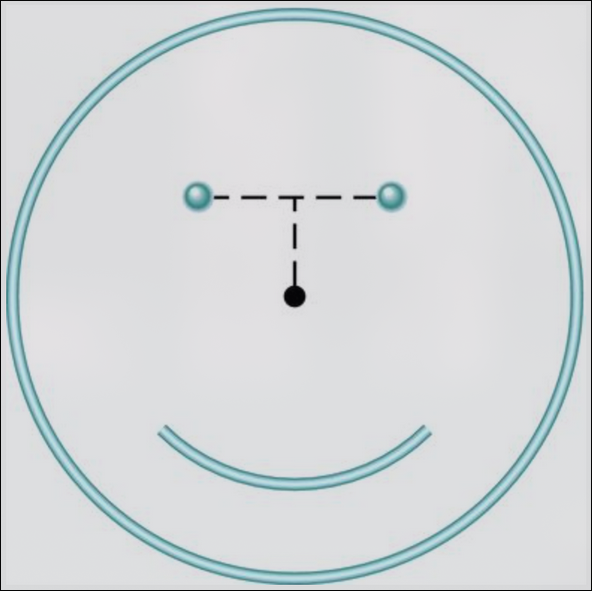
\includegraphics[width=0.5\textwidth]{image-8.png}
	\caption{Figure 24-49}
\end{figure}

\subsection*{Solution}
There is no field from the dipole because the dipole moment is perpendicular to the radial line. So we just have to find the potential from the two rods.
\begin{align*}
	V &= \frac{kq_1}{r} + \frac{kq_2}{4r} \\
	&= \frac{k(-3 \times 10^{-6})}{0.06} + \frac{k(2 \times 10^{-6})}{0.04} \\
\end{align*}
Notice that the ratios in the fractions are the same but of opposite sign so they just cancel out giving us $V = 0$.

\end{document}

